После победы в великой битве Король Ягуар хочет построить пирамиду, которая будет
одновременно монументом в честь победы и гробницей для погибших солдат. Пирамида
будет построена на поле боя. Она должна иметь прямоугольное основание, состоящее из $a$ столбцов и $b$ строк. Для сохранения останков и оружия павших солдат внутри основания пирамиды будет располагаться небольшая прямоугольная комната, состоящая из $c$ столбцов и $d$ строк.

Архитекторы Короля представили поле боя в виде прямоугольной сетки. Эта сетка состоит из квадратных клеток единичной площади и имеет $m$ столбцов и $n$ строк. Для каждой клетки они измерили ее высоту и получили некоторое целое число.

Основание пирамиды и комната должны покрывать включаемые ими клетки полностью, а их
стороны должны быть параллельны сторонам поля боя. Высоты клеток, составляющих
комнату, должны остаться неизменными, а высоты всех клеток основания пирамиды будут
выровнены с помощью перемещения песка с более высоких клеток на более низкие. В
результате этого высота основания пирамиды будет равна среднему арифметическому
высот всех его клеток (за исключением клеток комнаты). Архитекторы могут выбрать любое
местоположение для комнаты внутри пирамиды, но обязательно оставлять вокруг комнаты
стену основания пирамиды толщиной хотя бы в одну клетку.

Помогите архитекторам выбрать наилучшее место для расположения пирамиды и комнаты внутри нее так, чтобы высота основания пирамиды была максимально возможной при заданных размерах. На рисунке показан пример поля боя, где число в каждой клетке обозначает ее высоту. Клетки, составляющие основание пирамиды, обозначены серым цветом, а белые клетки внутри основания пирамиды соответствуют расположению комнаты. На этом рисунке представлен пример оптимального решения.

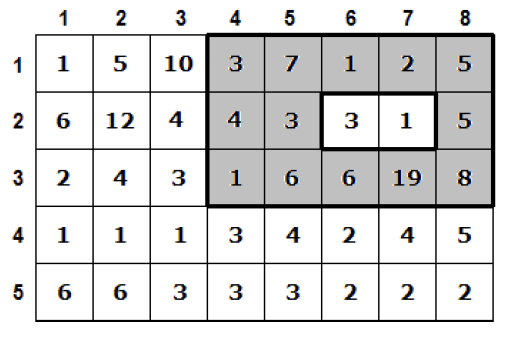
\includegraphics{piramida.png}


Напишите программу, которая по заданным размерам поля боя, пирамиды и комнаты, а
также по заданным высотам всех клеток будет находить такое расположение пирамиды и
комнаты внутри нее, что получившаяся высота основания пирамиды будет максимально
возможной. 